%% \begin{figure*}
%%       \centering
%%       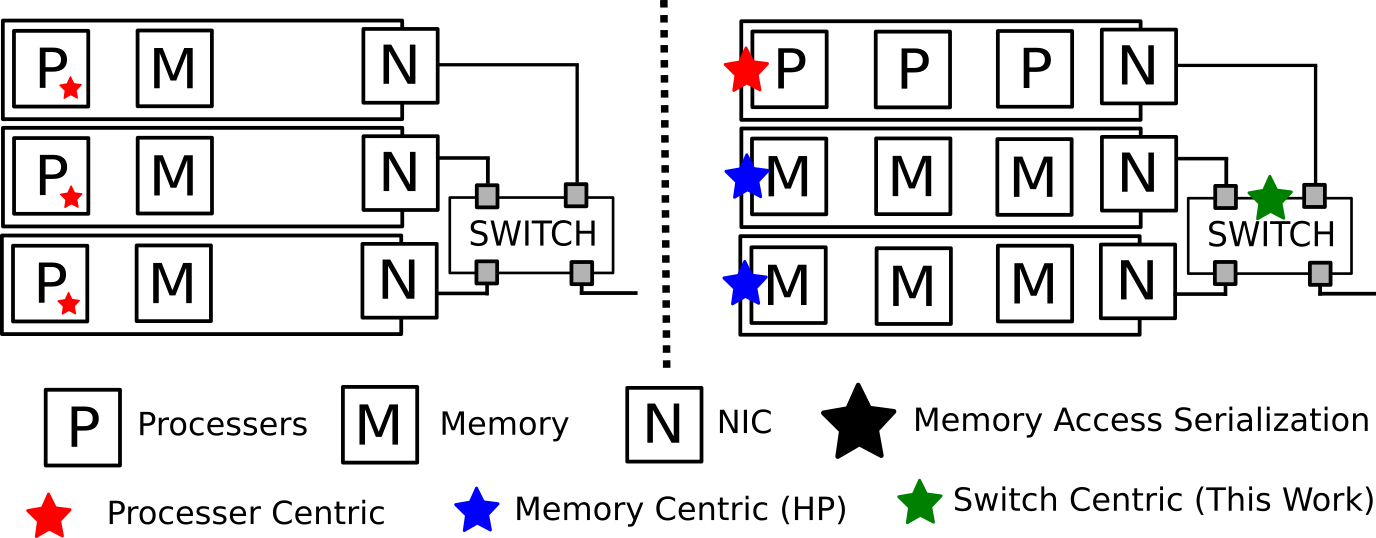
\includegraphics[width=0.95\textwidth]{fig/overview.png}
%%       %%
%%       \caption{~\todo{redo diagram to remove memory centric
%%       organization (it's a pipe dream)}
%%       Anatomy of a disaggregated rack. On the left a
%%       traditional rack with processors colocated with their memory
%%       interconnected by a switch. On the right is a high density
%%       disaggregated rack with processors separated from their memory
%%       by a top of rack switch. Stars mark locations for memory access
%%       serialization. Red denotes traditional processor centric
%%       serialization~\cite{memc3, cell, sonuma, storm, clover}, blue marks a
%%       memory centric architecture~\cite{aguilera2019designing}, and
%%       green marks a switch centric solution similar in spirit to
%%       proposed middle box solutions~\cite{254120}.
%%       \label{fig:overview}
%%       %%
%%       }
%% \end{figure*}


\section{In-network conflict resolution}

We propose a middle ground between a fully distributed and a
centralized approach. Our insight is that by using
data-structure-specific knowledge and caching metadata in the network,
conflicting writes can be resolved at line rate on the data path using
only a small amount of state. We use Clover as a platform to prove our
concept and design a middlebox algorithm which intercepts Clover's
RDMA read, write, and \texttt{c\&s} requests, caches a small amount
(64 bytes per key) of structural metadata, and resolves write
conflicts by adjusting the virtual destination address of contending
\texttt{c\&s} guards.

%Our system caches metadata for remote data structure on centralized
%networking devices. Our prototype is implemented in DPDK, however our
%algorithm could be implemented on a programmable switch or
%programmable NIC as long as it sees all requests to remote memory. 
%% kinds of devices
%A programmable TOR or our DPDK switch (which behaves as one) is ideal
%for rack scale disaggregated structures that potentially span multiple
%memory servers, while a programmable NIC implementation would be
%limited limited to the memory server it is attached to. 

%%Technique example
%The purpose of our technique is to resolve write conflicts to remote
%memory.

%As an illustrative example of a conflict consider a linked
%list implemented as a remote memory data structure with a single
%operation, \textit{appendTail}. 

%% This operation succeeds every time in the single threaded case as the
%% tail of the linked list is never moved by another process. Consider
%% instead the multi-threaded case in which two writers both attempt to
%% execute \textit{appendTail} concurrently. Both issue their first write
%% to remote memory successfully and then attempt to run an RDMA c\&s on
%% the tail of the old list. This results in a race condition where the
%% first process to write succeeds, and the other will fail. The process
%% which executes the c\&s second fails because rather than finding a tail
%% with a next value of NULL, it finds the now penultimate member of the
%% linked list which now points to the value issued by the process which
%% won the race. 

%% The process which lost the race now needs to engage in \textit{Pointer
%% chasing} to find the new tail. It must iterative issue reads of the
%% linked list, step by step until it finds the location of the new tail.
%% At which point it can reissue a c\&s to make the new tail point to it's
%% value. The reissued c\&s is also subject to the same race condition as
%% many writers may be execution \textit{appendTail}. This reconciliation
%% algorithm of pointer chasing must be run each time a conflict occurs.
%% For highly contested structures, the number of retries can grow
%% quickly, leading to large and unpredictable tail latencies.

%% In the case of clover this exact scenario occurs when key are write
%% contested. Their experiments with a zipf distribution on their keys
%% sees a 5x reduction in throughput at 50\% writes.

%% What do we actually do

\subsection{Resolving concurrent requests}

Our key observation is that a top-of-rack (TOR) switch necessarily
serializes all RDMA operations destined to any particular remote memory
location, since physical memory is hosted on a single server, and the
switch is in charge of ordering packets destined to each of its output
ports.  (We leave the engineering details involved in addressing
multi-homed servers, corrupt packets, node failures, and the like to
future work.)  Given an ordered stream of RDMA operations, it is
straightforward for an in-network device to detect stale \texttt{c\&s}
operations.  What's more, if the TOR maintains just a modest amount of
state, it can resolve conflicts in flight.  Specifically, it suffices
to redirect any \texttt{c\&s} operations that ``lost their races'' to the
address of the current (or soon-to-be) end of the chain.
%%

%% Our observation is that such a coordinator can be implemented in
%% network can significantly improve throughput. Using data structure
%% specific information the coordinator can cache recent writes, and
%% steer concurrent ones to locations which will result in successful
%% operations and maintain the correctness of the remote data structure.

%Clover maintains versioning information in the form
%of a linked list which operates identically to the \textit{appendTail}
%operation described above.

In the particular case of Clover, we cache the current end of the
chain for each key in Clover's key/value store. This requires $O(n)$
state where $n$ is the number of keys. For a key/value store
consisting of ten-thousand keys we need to store a key mapping and
value for each (both 64 bits) resulting in a total in-network storage
of 80~KB.  Note that this represents only a small portion of the
metadata Clover maintains at its metadata servers which contains all
versions on the chain. Only the end of the chain is required to
resolve write conflicts.


\subsection{Modifying RDMA in flight}

Interposing on the RDMA protocol, however, is non-trivial. One approach
(evaluated in Clover as pDPM-central~\cite{clover}) employs an RDMA-enabled
middlebox that sets up connections between itself and clients and another set
of connections to the memory servers. The middlebox can then reorder, rewrite,
and relay RDMA requests from clients to the appropriate chain locations. This
solution is impractical for a TOR-based solution both because existing
switches lack the ability to establish RDMA connections, and, more
importantly, because the authors of Clover demonstrate it to be a
performance bottleneck. We avoid both shortcomings by transparently
intercepting RDMA connections established directly between the clients and
remote memory servers without explicitly participating in the RDMA protocol.

In our approach, the TOR records the virtual addresses used in any
RDMA writes made by Clover clients. These writes are marked as
\textit{outstanding}; i.e., they have been issued to remote memory,
but have not yet been made visible in Clover because they are not yet
connected to Clover's per-key chain.  As described above, following
the completion of an outstanding write, clients issue an RDMA \texttt{c\&s} to
the end of the chain to make their update visible atomically in
Clover, and we also track the last \texttt{c\&s} issued for each key.  In a
successful update, the \texttt{c\&s} operation will adjust the next-update
pointer to the location of the most recent (outstanding) write,
thereby committing the write.

Our algorithm detects the existence of a conflict by noticing when
there are multiple outstanding writes for a given key. The current
write for each client is tracked, when two clients have outstanding
writes to the same key a conflict has occurred. When a \texttt{c\&s}
operation arrives, we inspect the virtual address it is trying to
update. If it points to an old tail, its virtual address is modified
by the TOR (without the knowledge of the issuing client) to point to
the true tail of the list. The cached latest version of the key is
then updated to point to the address to which the \texttt{c\&s} was
directed. Clover clients learn the updated locations using their
default read algorithm.

\subsection{Prototype}

Our prototype is implemented in a software switch using DPDK, but is
designed to have low memory and computational overhead making it ideal
for network devices such as programmable switches.  RDMA packets are
not intended to be modified in flight, and care must be taken not to
corrupt them. RDMA invariant CRCs (ICRC) are calculated at the time of
sending and are designed to ensure the integrity of the payload. When
we modify \texttt{c\&s} packets their ICRC must be recalculated or the packet
will be rejected by the receiving NIC. FPGA implementations of RDMA
ICRC have been built in the past~\cite{Mansour_2019}; the required CRC
calculation is identical to Ethernet CRC, with some additional header
components and field masking.
%Our DPDK solution uses \texttt{zlib}'s
%\texttt{crc32} for the calculation.
%We believe that
%this algorithm can also be implemented efficiently on a programmable
%switch.


